% !TeX root = ../document_main.tex
% ============================================================
% 6. Alignment with International Standards
% ============================================================

\begin{sectionintro}{6}{Alignment with International Standards}{
  \begin{itemize}[leftmargin=1.5em]
    \item Zero Trust Architecture --- NIST SP 800-207
    \item NIST SP 800-53 Rev.\ 5 security controls
    \item PCI DSS v4.0 cardholder data protection
    \item HIPAA Security Rule for healthcare data
    \item GDPR data protection by design
    \item ISO/IEC 27001:2022 information security management
    \item CCPA consumer privacy rights enforcement
    \item SOC 2 Type II trust services criteria
    \item Cryptographic standards (FIPS 197, RFC 8446, FIPS 186-4)
    \item OWASP Top 10 mitigation coverage
  \end{itemize}
}
Compliance with international security standards is a foundational design objective for zGate rather than an afterthought applied after implementation. Six regulatory frameworks --- HIPAA, GDPR, ISO/IEC 27001, PCI DSS, CCPA, and SOC 2 Type II --- are natively catalogued in the system's compliance engine (\path{internal/compliance/catalog.go}), with prescriptive safety templates, query-blocking rules, and AI-driven masking policies that are seeded automatically at server startup and directly enforced at the protocol layer. This chapter traces each architectural and cryptographic decision to its governing international standard, demonstrating that zGate's control surface inherently satisfies the access control, audit, encryption, and data-protection obligations of the major international regulatory frameworks.
\end{sectionintro}

% ──────────────────────────────────────────────────────────────────────────────
\section{Zero Trust Architecture --- NIST SP 800-207}
% ──────────────────────────────────────────────────────────────────────────────

NIST Special Publication 800-207 defines Zero Trust Architecture (ZTA) as a collection of concepts and ideas designed to minimise uncertainty in enforcing accurate, least-privilege per-request access decisions in information systems and services~\cite{nist-zt}. The standard identifies three core tenets: \textit{verify explicitly}, \textit{use least-privilege access}, and \textit{assume breach}. zGate implements all three tenets directly at the database protocol layer.

\subsection{Tenet 1 --- Verify Explicitly}

Every database connection attempt requires active cryptographic verification. The gateway supports two distinct authentication paths:

\begin{itemize}
    \item \textbf{JWT Bearer Path:} Users authenticate via the REST login endpoint and receive a signed JSON Web Token (HMAC-SHA256, 5-minute access token + 1-hour rotating refresh token stored as a SHA-256 hash). Before any TCP tunnel is opened, the server validates the token signature, evaluates the \texttt{exp} and \texttt{jti} claims against a revocation table, and re-reads the user's current role permissions directly from the encrypted store --- not from stale token claims.
    \item \textbf{mTLS Certificate Path:} Service accounts authenticate using ECDSA P-256 client certificates issued by the internal Certificate Authority (\path{internal/pki/ca.go}). The gateway listener enforces TLS~1.3 as the minimum protocol version, verifies the full certificate chain against the CA trust pool, validates that the leaf certificate carries \texttt{ExtKeyUsageClientAuth}, consults the real-time revocation cache, and checks the source IP against a per-certificate CIDR allowlist --- all before a single database byte is exchanged.
\end{itemize}

\subsection{Tenet 2 --- Least-Privilege Access}

Access decisions are computed fresh on every connection request. The Policy Engine (\path{internal/policy/engine.go}) reads the user's current role assignments and per-database permission levels directly from the live store; no cached permission set from a JWT is trusted. Users are granted access only to the specific named databases their roles entitle them to, with permission levels scoped to \textit{read}, \textit{read-write}, or \textit{admin}. Token-bucket rate limiting further constrains query volume per user per database, preventing bulk data extraction even by legitimately authenticated users.

\subsection{Tenet 3 --- Assume Breach}

The assume-breach pillar is addressed by layered controls that operate even when perimeter defences have been bypassed:

\begin{itemize}
    \item \textbf{Credential Abstraction:} Users are never issued the real database password. The gateway rewrites authentication credentials at the wire-protocol level (\path{internal/proxy/credentials/}), so a stolen session ticket cannot be used to connect directly to the backend database.
    \item \textbf{ML-Based Anomaly Detection:} Every query is scored post-execution by a sidecar anomaly service that extracts structural AST features (table count, join depth, presence of WHERE/LIMIT, subquery depth, column selection breadth) and assigns a severity rating. Critical and high-severity anomalies are persisted and surfaced to administrators in real time (\path{internal/proxy/interceptor/anomaly.go}).
    \item \textbf{Immutable Audit Trail:} Every query --- including session ID, user identity, client IP, SQL text, query type, affected tables, row count, and anomaly metadata --- is written to a rotating JSON audit log and simultaneously emitted to OpenTelemetry for forwarding to external SIEM systems.
    \item \textbf{Session Revocation:} Administrators can forcibly terminate active sessions from the admin panel, which immediately invalidates the in-flight session; subsequent queries on the revoked session produce an authentication error at the gateway boundary.
\end{itemize}

% ──────────────────────────────────────────────────────────────────────────────
\section{NIST SP 800-53 Rev.\ 5 --- Security and Privacy Controls}
% ──────────────────────────────────────────────────────────────────────────────

NIST SP 800-53 Revision 5 provides a comprehensive catalogue of security and privacy controls for federal information systems and organisations~\cite{nist-controls}. Table~\ref{tab:nist-controls} maps zGate's implementation to the relevant control families.

\renewcommand{\arraystretch}{1.3}
\small
\setlength\LTleft\fill
\setlength\LTright\fill
\begin{table}[H]
\caption{zGate implementation mapped to NIST SP 800-53 Rev.\ 5 controls}
\label{tab:nist-controls}
\begin{tabular}{|p{1.6cm}|p{4.0cm}|p{9cm}|}
\hline
\textbf{Control} & \textbf{Family} & \textbf{zGate Implementation} \\
\hline
AC-2 & Account Management & Admin accounts provisioned with mandatory role and tier assignment; service accounts issued with configurable certificate validity \\
\hline
AC-3 & Access Enforcement & Policy Engine performs per-request live permission lookup; stale cached claims are never trusted \\
\hline
AC-6 & Least Privilege & Users receive only the permission level (read / read-write / admin) explicitly assigned per database \\
\hline
AC-7 & Unsuccessful Logon Attempts & ALTCHA proof-of-work (500k SHA-256 iterations) and HTTP rate limiting protect the login endpoint \\
\hline
AC-12 & Session Termination & 5-minute JWT expiry; admin-initiated forced session revocation; JTI blacklisting \\
\hline
AU-2 & Event Logging & All queries, auth events, session starts/ends, policy violations, and anomalies are logged \\
\hline
AU-3 & Content of Audit Records & Each record includes username, session ID, client IP, database, protocol, SQL text, query type, tables/columns, duration, safety status, anomaly score, and OTel trace ID \\
\hline
AU-9 & Protection of Audit Information & Log files use \texttt{lumberjack} rotation; control-plane store encrypted AES-256-GCM; OTel export provides off-system copy \\
\hline
IA-2 & Identification \& Authentication & Every user uniquely identified by \texttt{account\_id} in JWT; no anonymous login \\
\hline
IA-2(1) & Multi-Factor Authentication & TOTP (RFC 6238) available for all administrative accounts \\
\hline
IA-3 & Device Identification & Service accounts authenticate via ECDSA P-256 client certificates tracked by SHA-256 fingerprint \\
\hline
IA-5 & Authenticator Management & Refresh tokens stored only as SHA-256 hashes; secrets encrypted AES-256-GCM; Vault integration for secret delivery \\
\hline
IA-8 & Non-Org User Authentication & OIDC integration with Keycloak (\path{internal/auth/oidc.go}) enables federated identity via OpenID Connect \\
\hline
SC-8 & Transmission Confidentiality & All gateway connections enforce TLS~1.3; session ticket resumption disabled \\
\hline
SC-12 & Cryptographic Key Management & CA private key encrypted with store master key; secrets loaded from HashiCorp Vault via AppRole \\
\hline
SC-28 & Protection of Information at Rest & MySQL control-plane store encrypted AES-256-GCM with 128-bit random nonce per operation \\
\hline
SI-4 & System Monitoring & Anomaly detection flags suspicious patterns; OpenTelemetry metrics export continuous observability data \\
\hline
SI-10 & Information Input Validation & All API inputs pass through the validation layer; SQL queries are AST-parsed before forwarding \\
\hline
\end{tabular}
\end{table}
\renewcommand{\arraystretch}{1}

% ──────────────────────────────────────────────────────────────────────────────
\section{Payment Card Industry Data Security Standard (PCI DSS v4.0)}
% ──────────────────────────────────────────────────────────────────────────────

The PCI DSS version 4.0, published by the PCI Security Standards Council in 2022, mandates technical and operational controls for any system that stores, processes, or transmits cardholder data within the Cardholder Data Environment (CDE)~\cite{pci-dss-v4}. zGate's built-in PCI DSS compliance framework provides a native enforcement layer for the most security-critical PCI requirements.

\begin{figure}[H]
    \centering
    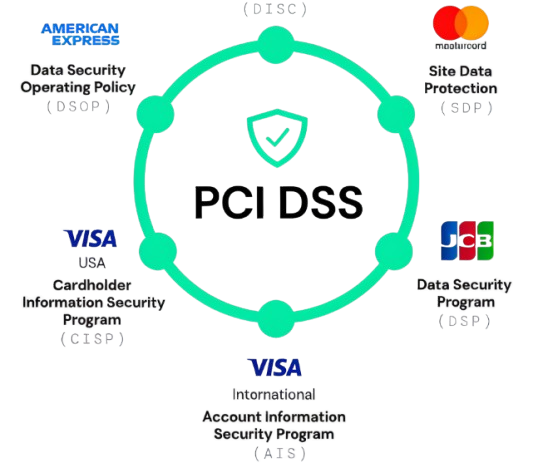
\includegraphics[width=0.55\textwidth]{images/PCI-DSS.png}
    \caption{zGate alignment with PCI DSS v4.0 requirements for CDE access control, authentication, and audit logging}
    \label{fig:pci-dss-compliance}
\end{figure}

\subsection{Requirement 3 --- Protect Stored Account Data}

PCI DSS Requirement 3 mandates that Primary Account Numbers (PANs) must be rendered unreadable wherever stored. zGate's \textit{PCI DSS --- Cardholder Data Auto-Mask} AI template automatically detects PAN columns in query results and applies the \texttt{last4} masking strategy, which is explicitly compliant with PCI DSS Requirement 3.3 (``Display only the first six and/or last four digits of the PAN as the maximum number of digits to be displayed'')~\cite{pci-dss-v4}. Database credentials in the control plane are encrypted with AES-256-GCM per Requirement 3.5.

\subsection{Requirement 6 --- Develop and Maintain Secure Systems}

The \textit{PCI DSS --- Block Dangerous Functions} safety template prevents SQL injection exploitation at the query-interception layer: calls to \texttt{SLEEP}, \texttt{BENCHMARK}, \texttt{LOAD\_FILE}, and \texttt{INTO OUTFILE} are rejected before reaching the backend database, satisfying Requirement 6.3 injection prevention~\cite{pci-dss-v4}. The \textit{PCI DSS --- Block System Schema Access} template prevents metadata enumeration via \texttt{DESCRIBE} and \texttt{information\_schema} queries per Requirement 6.4.

\subsection{Requirement 7 --- Restrict Access to System Components and Cardholder Data}

The \textit{PCI DSS --- CDE Strict Access Control} safety template operates in \textbf{strict enforcement mode}: only explicitly whitelisted query patterns (bounded SELECT with WHERE, no wildcard columns, LIMIT~$\leq 50$) are permitted; all other query types are blocked by default. Moderate-bound SELECTs (LIMIT 51--200) are flagged for human review before proceeding. This satisfies the need-to-know access control principle of Requirement 7.1. The RBAC Policy Engine ensures that only users with explicit per-database permissions can initiate connections.

\subsection{Requirement 8 --- Identify Users and Authenticate Access}

\begin{itemize}
    \item \textbf{Req.\ 8.2 --- Unique User IDs:} Every user is assigned a unique \texttt{account\_id} embedded in their JWT; shared usernames are prohibited by a database schema constraint.
    \item \textbf{Req.\ 8.3 --- Strong Authentication:} TOTP-based multi-factor authentication is supported for all administrative accounts. JWT access tokens expire after 5 minutes; stolen tokens cannot be replayed beyond their expiry window.
    \item \textbf{Req.\ 8.6 --- System and Application Accounts:} Service accounts authenticate via ECDSA P-256 certificates with configurable expiry; each certificate is individually tracked in the revocation cache.
    \item \textbf{Req.\ 8.8 --- No Shared Credentials:} Users connect via session-specific ephemeral or personal credentials generated by the gateway's credential provisioner. No user ever handles or transmits a shared backend database password.
\end{itemize}

\subsection{Requirement 10 --- Log and Monitor All Access to System Components}

The \textit{PCI DSS --- Flag Batch Queries for Review} template flags multi-statement queries against CDE databases for Requirement 10.6 anomalous-activity review. All database access events are logged with user identity, timestamp (RFC~3339), session ID, query text, and safety status, satisfying the audit-record content requirements of Requirements 10.2--10.3. Anomaly scores are embedded in every log record to support the suspicious-activity identification requirement of Requirement 10.6.

% ──────────────────────────────────────────────────────────────────────────────
\section{HIPAA Security Rule}
% ──────────────────────────────────────────────────────────────────────────────

The HIPAA Security Rule (45 CFR Part 164) imposes administrative, physical, and technical safeguards on Covered Entities and Business Associates that create, receive, maintain, or transmit Electronic Protected Health Information (ePHI)~\cite{hipaa-security-rule}. zGate's built-in HIPAA compliance framework enforces the technical safeguards directly at the database query layer, independent of application-layer changes.

\subsection{Technical Safeguards (45 CFR \S~164.312)}

\begin{itemize}
    \item \textbf{Access Control (\S~164.312(a)(1)):} Role-based permissions restrict each user to only the databases containing ePHI they are authorised to access. The Policy Engine re-evaluates entitlements on every connection request without trusting cached credential data.
    \item \textbf{Automatic Log-off (\S~164.312(a)(2)(iii)):} JWT access tokens automatically expire after 5 minutes. Administrators can force-terminate any active session immediately from the admin panel, ensuring that unattended sessions are not exploitable.
    \item \textbf{Audit Controls (\S~164.312(b)):} Every database query executed against an ePHI database is captured with a complete audit record, including the user's identity, timestamp, query text, and the specific tables accessed. Records are immutable after creation and exported to OpenTelemetry for off-system retention.
    \item \textbf{Person or Entity Authentication (\S~164.312(d)):} TOTP multi-factor authentication is available for all administrative accounts. The OIDC integration enables organisation-wide identity verification through Keycloak.
    \item \textbf{Transmission Security (\S~164.312(e)(1)):} All connections to the gateway are protected with TLS~1.3. Credential injection from the gateway to the backend database occurs over encrypted database protocol connections.
\end{itemize}

\subsection{HIPAA Minimum Necessary and Safe Harbor Data Masking}

The \textit{HIPAA --- Block Unbounded Queries} safety template enforces the Minimum Necessary standard (\S~164.502(b)) by rejecting SELECT statements that lack a WHERE clause, preventing bulk ePHI extraction. The \textit{HIPAA --- Restrict Destructive Operations} template blocks DELETE, DROP, and TRUNCATE to protect ePHI retention requirements. Schema modification via ALTER and DROP is blocked to prevent attackers from circumventing column-level masking rules.

The \textit{HIPAA --- PHI Auto-Mask} AI masking template automatically identifies and masks all 18 Safe Harbor identifier categories defined in 45 CFR \S~164.514(b)(2) --- including names, geographic subdivisions, dates, telephone numbers, email addresses, social security numbers, account numbers, and IP addresses --- inline in query results before data is returned to the client, without requiring any changes to application code.

% ──────────────────────────────────────────────────────────────────────────────
\section{General Data Protection Regulation (GDPR)}
% ──────────────────────────────────────────────────────────────────────────────

The GDPR (EU 2016/679) establishes data protection rights for EU data subjects and imposes strict obligations on controllers and processors of personal data, with particular emphasis on Privacy by Design and by Default under Article 25~\cite{gdpr-2016}.

\begin{figure}[H]
    \centering
    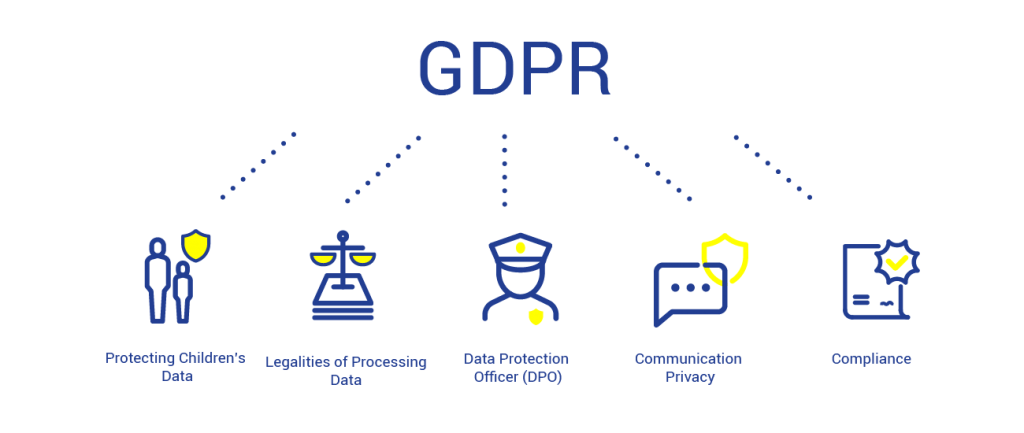
\includegraphics[width=0.7\textwidth]{images/GDPR.png}
    \caption{zGate alignment with GDPR requirements for data security, access control, audit records, and breach detection}
    \label{fig:gdpr-compliance}
\end{figure}

\subsection{Article 5(1)(f) --- Integrity and Confidentiality}

Personal data must be processed with appropriate security against unauthorised or unlawful processing and against accidental loss or destruction. zGate satisfies this principle through: AES-256-GCM encryption of the control-plane store; TLS~1.3 for all gateway connections; ECDSA P-256 mutual TLS authentication for service accounts; and query-level masking of PII columns before data reaches the client.

\subsection{Article 25 --- Data Protection by Design and by Default}

Article 25 requires that data protection principles be integrated into processing activities by design, and that only data necessary for each specific purpose be processed by default. zGate enforces this through:
\begin{itemize}
    \item The \textit{GDPR --- Block Unbounded PII Queries} template blocks SELECT statements without a WHERE clause, enforcing data minimisation at the database layer.
    \item The \textit{GDPR --- Flag Bulk SELECT for Review} template intercepts wildcard column selections for human review before bulk PII is returned to any caller.
    \item The \textit{GDPR --- PII Auto-Mask} AI template automatically detects and masks PII fields (email, phone, full name, IP address, date of birth, address, SSN) in query results across MySQL, PostgreSQL, and MSSQL, without requiring changes to application code.
    \item Cross-region data access is controlled by the \textit{GDPR --- Block Cross-Region Table Access} template, which blocks access to configured restricted schemas to enforce tenant isolation between GDPR data residency zones.
\end{itemize}

\subsection{Article 30 --- Records of Processing Activities}

Controllers are required to maintain records of processing activities under Article 30(1). Every SQL query executed through zGate is logged with user identity, session ID, timestamp (RFC~3339), database name, query type, affected tables, and execution duration. These structured JSON records --- together with role assignments stored in the control-plane --- provide the purpose, category, and processing-activity documentation required by Article 30.

\subsection{Article 32 --- Security of Processing}

Article 32 requires controllers to implement appropriate technical measures including pseudonymisation, encryption, and ongoing assessment of data security. zGate delivers:
\begin{itemize}
    \item \textbf{Encryption:} AES-256-GCM at rest; TLS~1.3 in transit.
    \item \textbf{Pseudonymisation:} Fake-data masking strategies (\texttt{fake\_name}, \texttt{fake\_email}, \texttt{fake\_phone}, \texttt{fake\_address}, \texttt{fake\_ssn}) replace real PII with structurally valid synthetic values, preserving referential integrity for development and analytics workflows while removing identifiability.
    \item \textbf{Ongoing Confidentiality and Integrity:} HMAC-SHA256 signs ALTCHA challenges; anomaly detection provides continuous assessment of access patterns.
    \item \textbf{Availability:} The anomaly detection service uses a fail-open timeout pattern: its unavailability does not interrupt database access, ensuring that the security control does not compromise availability.
\end{itemize}

\subsection{Article 33 --- Notification of Personal Data Breach}

Article 33 requires Controllers to notify the supervisory authority of a personal data breach within 72 hours of becoming aware of it. The anomaly detection subsystem flags high-severity and critical-severity query patterns in real time and persists notifications containing the offending query, session ID, user identity, anomaly score, severity, and OpenTelemetry correlation ID. These structured records provide the evidence base required to assess notification obligations and demonstrate due diligence. The \textit{GDPR --- Restrict DELETE to Authorised Roles} template enforces the Right to Erasure (Article 17) by blocking unauthorised DELETE operations.

% ──────────────────────────────────────────────────────────────────────────────
\section{ISO/IEC 27001:2022 --- Information Security Management}
% ──────────────────────────────────────────────────────────────────────────────

ISO/IEC 27001:2022 is the international standard for Information Security Management Systems (ISMS), specifying requirements for establishing, implementing, maintaining, and continually improving an ISMS~\cite{iso27001-2022}. Annex A of the 2022 revision defines 93 information security controls organised into four themes. zGate provides direct technical implementation for the following Annex A controls.

\subsection{Organisational Controls (Annex A.5)}

\begin{itemize}
    \item \textbf{A.5.15 --- Access Control:} Policies and rules for controlling access to information and associated assets are enforced at the database protocol layer through the RBAC Policy Engine, which re-evaluates entitlements on every connection request.
    \item \textbf{A.5.17 --- Authentication Information:} Authenticator information (database credentials, refresh token hashes, TOTP secrets) is stored exclusively as AES-256-GCM ciphertext or SHA-256 hashes; plaintext credentials are never persisted in any store.
\end{itemize}

\subsection{Technological Controls (Annex A.8)}

\begin{itemize}
    \item \textbf{A.8.2 --- Privileged Access Rights:} The admin tier model (super / db\_admin / policy\_admin / auditor) ensures that privileged capabilities are assigned on a need-to-have basis, are separately auditable, and cannot be self-escalated.
    \item \textbf{A.8.3 --- Information Access Restriction:} Access is restricted to users with explicit per-database permissions. The ISO~27001 safety templates enforce column-level restriction by blocking wildcard SELECT and blocking DESCRIBE metadata probing, enforcing the A.9.4 minimum-necessary principle.
    \item \textbf{A.8.15 --- Logging:} All system activities, results, and user actions are captured in structured audit records containing unique session identifiers and OpenTelemetry trace/span IDs for distributed correlation.
    \item \textbf{A.8.16 --- Monitoring Activities:} The anomaly detection subsystem provides continuous behavioural monitoring of SQL traffic. Metrics (query rate, rate-limit rejections, active sessions) are exported to Prometheus-compatible collectors via the OpenTelemetry SDK.
    \item \textbf{A.8.24 --- Use of Cryptography:} The cryptographic policy is implemented consistently: AES-256-GCM for symmetric encryption, ECDSA P-256 for asymmetric operations, SHA-256 / HMAC-SHA256 for integrity and authentication challenges, and TLS~1.3 for transport security.
    \item \textbf{A.8.25 --- Secure Development Lifecycle:} Security controls (query analysis, masking, anomaly detection, rate limiting) are integrated into the application's request-processing pipeline as composable interceptors, not bolted on externally. Each interceptor can be independently versioned, tested, and deployed without modifying the proxy core.
\end{itemize}

\subsection{Built-in ISO/IEC 27001 Safety Templates}

The compliance engine (\path{internal/compliance/catalog.go}) includes five ready-to-apply ISO~27001 safety templates:
\begin{enumerate}
    \item \textit{Block Unbounded Queries:} enforces A.9.4 minimum-necessary access with tiered LIMIT thresholds --- allow $\leq 100$, warn 101--500, block $> 500$ rows.
    \item \textit{Block Wildcard SELECT:} rejects \texttt{SELECT *} per A.9.4.
    \item \textit{Block System Schema Access:} prevents \texttt{information\_schema} enumeration per A.12.3 data integrity.
    \item \textit{Restrict Destructive Operations:} blocks DELETE, DROP, and TRUNCATE per A.12.3.
    \item \textit{Flag Privileged Operations for Review:} flags ALTER, CREATE, GRANT, and REVOKE for A.9.2 access-management audit review.
\end{enumerate}

% ──────────────────────────────────────────────────────────────────────────────
\section{California Consumer Privacy Act (CCPA)}
% ──────────────────────────────────────────────────────────────────────────────

The CCPA (Cal.\ Civ.\ Code \S\S~1798.100--1798.199), effective January 2020 and strengthened by the California Privacy Rights Act (CPRA) in 2023, grants California residents rights over their personal information and imposes security obligations on qualifying businesses~\cite{ccpa-2018}.

\begin{itemize}
    \item \textbf{\S~1798.100/110 --- Right of Access and Disclosure:} Audit logs provide a complete record of which users accessed which Personal Information (PI) categories, enabling businesses to respond to consumer access requests with a verifiable data-access history including timestamp, user identity, and specific tables queried.
    \item \textbf{\S~1798.105 --- Right to Delete:} The \textit{CCPA --- Restrict DELETE to Authorised Roles} template ensures that PI deletion is restricted to explicitly authorised personnel, preventing both unauthorised erasure and the bypassing of consent-based deletion workflows.
    \item \textbf{\S~1798.140(o) --- Personal Information Definition:} The \textit{CCPA --- Personal Information Auto-Mask} template automatically detects and masks CCPA-defined PI categories in query results --- including email, phone, full name, SSN, address, IP address, and date of birth --- using the AI column classification subsystem.
    \item \textbf{\S~1798.100 --- Bulk Export Prevention:} The \textit{CCPA --- Block INTO OUTFILE Exports} template prevents direct file-system exports that bypass all access controls. The \textit{CCPA --- Flag Bulk PI Exports for Review} template intercepts wildcard SELECT statements for human approval, preventing mass PI extraction that would undermine consumer rights.
    \item \textbf{\S~1798.150 --- Data Security:} The combination of AES-256-GCM encryption, TLS~1.3 transport security, multi-factor authentication, and comprehensive audit logging satisfies the ``reasonable security procedures and practices'' standard required by CCPA \S~1798.150.
\end{itemize}

% ──────────────────────────────────────────────────────────────────────────────
\section{SOC 2 Type II --- Trust Services Criteria}
% ──────────────────────────────────────────────────────────────────────────────

SOC 2 Type II is governed by the American Institute of Certified Public Accountants (AICPA) Trust Services Criteria (TSC) and provides an audit framework demonstrating that a service organisation's security controls are effective over a sustained observation period~\cite{soc2-2022}. Unlike SOC 2 Type I (which attests to control design), Type II requires that controls operate consistently throughout the audit window --- an objective directly supported by the compliance engine's startup-seeded, administratively-protected templates.

\begin{itemize}
    \item \textbf{CC6.1 --- Logical and Physical Access Controls:} The \textit{SOC 2 --- Logical Access Control} strict-mode template enforces that only bounded SELECT queries (WHERE, no wildcard, LIMIT~$\leq 100$) are allowed; all other query patterns are blocked by default. This boundary is demonstrably auditable.
    \item \textbf{CC6.2 --- Access Provisioning:} Role assignments, permission levels, and certificate issuances are performed through the admin API with full audit records. The \textit{SOC 2 --- Flag Privilege Escalation Attempts} template flags GRANT and REVOKE operations for CC6.2 provisioning review.
    \item \textbf{CC6.3 --- Access Removal:} The admin panel supports instant session revocation and per-certificate revocation. JTI blacklisting prevents reuse of revoked JWT access tokens even within their 5-minute lifetime.
    \item \textbf{CC6.6 --- Logical Access Security from Threats:} The \textit{SOC 2 --- Block System Enumeration} template blocks system-schema access to reduce the external attack surface. ALTCHA proof-of-work and HTTP rate limiting protect the authentication endpoint against automated credential-stuffing attacks.
    \item \textbf{CC7.2 --- Monitoring of System Components:} OpenTelemetry-based metrics and distributed tracing provide continuous monitoring. The anomaly detection subsystem continuously evaluates query patterns for deviations from expected behaviour and surfaces alerts.
    \item \textbf{CC8.1 --- Change Management:} The \textit{SOC 2 --- Flag Schema Changes} template flags ALTER and CREATE statements as CC8.1 change-management events requiring documentation, producing an auditable trail of schema modifications throughout the audit observation period.
\end{itemize}

% ──────────────────────────────────────────────────────────────────────────────
\section{Cryptographic Standards Compliance}
% ──────────────────────────────────────────────────────────────────────────────

All cryptographic primitives used in zGate conform to NIST-approved algorithms and published RFCs. Table~\ref{tab:crypto-standards} summarises each primitive, its specific usage, and its governing standard.

\begin{table}[H]
\small
\centering
\renewcommand{\arraystretch}{1.4}
\begin{tabularx}{\textwidth}{|p{2.8cm}|X|p{3.0cm}|p{3.5cm}|}
\hline

\textbf{Primitive} & \textbf{Usage in zGate} & \textbf{Standard} & \textbf{Key / Digest Size} \\
\hline
AES-GCM & Control-plane store encryption; service-account secret encryption & FIPS 197~\cite{fips-197} & 256-bit key \\
\hline
ECDSA & Internal CA key pair; client and server certificate signing & FIPS 186-4~\cite{fips-186-4} & P-256 curve \\
\hline
TLS 1.3 & Gateway TCP listener; REST API transport & RFC 8446~\cite{tls13} & Protocol \\
\hline
SHA-256 & Certificate fingerprinting; refresh-token hashing; ALTCHA PoW solution; HMAC basis & FIPS 180-4~\cite{fips-180-4} & 256-bit digest \\
\hline
HMAC-SHA256 & ALTCHA challenge signing; puzzle signing to prevent tampering & RFC 2104~\cite{rfc-2104} & $\geq$256-bit key \\
\hline
HS256 (HMAC-SHA256) & JWT access and refresh token signing & RFC 7519~\cite{rfc-7519} & $\geq$256-bit key \\
\hline
CSPRNG & AES-GCM nonce; certificate serial numbers; refresh tokens; JWT JTI & \texttt{crypto/rand} (Go) & 128-bit entropy \\
\hline
TOTP & Admin multi-factor authentication & RFC 6238~\cite{rfc-6238} & SHA-1 / 30-second window \\
\hline
\end{tabularx}
\caption{Cryptographic primitives used in zGate and their governing standards}
\label{tab:crypto-standards}
\end{table}

Certificate serial numbers are generated as 128-bit cryptographically random integers using Go's \texttt{crypto/rand} CSPRNG, satisfying both the CA/Browser Forum entropy recommendations and NIST SP 800-57 guidance on randomness for certificate serial number generation~\cite{nist-key}. Session ticket resumption is explicitly disabled in the mTLS listener (\texttt{SessionTickets\-Disabled:~true}) to prevent a revoked certificate from bypassing the revocation cache through a TLS session resumption.

% ──────────────────────────────────────────────────────────────────────────────
\section{OWASP Top 10 Mitigations}
% ──────────────────────────────────────────────────────────────────────────────

The OWASP Top 10 (2021) represents the most critical web and application security risk categories~\cite{owasp-top10}. zGate addresses the database-relevant categories as follows:

\begin{itemize}
    \item \textbf{A01:2021 --- Broken Access Control:} The RBAC Policy Engine performs per-request fresh permission checks; no cached claim is trusted for access decisions. The mTLS gateway enforces ExtKeyUsage validation, IP allowlisting, and real-time revocation cache checks, ensuring that a compromised certificate cannot be reused after revocation.
    \item \textbf{A02:2021 --- Cryptographic Failures:} AES-256-GCM is used with a cryptographically random 128-bit nonce per encryption operation, preventing nonce reuse attacks. TLS~1.3 with session ticket resumption disabled prevents protocol downgrade and session-resumption-based revocation bypass.
    \item \textbf{A03:2021 --- Injection:} SQL queries are parsed into an abstract syntax tree before forwarding. Dangerous functions (\texttt{SLEEP}, \texttt{BENCHMARK}, \texttt{LOAD\_FILE}, \texttt{INTO OUTFILE}) are detected and blocked at the interceptor layer, preventing time-based blind injection and file-system exploitation. System-schema access is blocked to cut off metadata-based injection reconnaissance.
    \item \textbf{A07:2021 --- Identification and Authentication Failures:} Short-lived JWT tokens (5-minute expiry), TOTP MFA, ALTCHA proof-of-work (500k SHA-256 iterations), HTTP rate limiting, and mTLS client certificates for service accounts comprehensively address credential stuffing, brute-force, and token-replay attack vectors.
    \item \textbf{A09:2021 --- Security Logging and Monitoring Failures:} Every query is logged with a complete audit record and simultaneously emitted to OpenTelemetry for external SIEM integration. Anomaly scores, severity ratings, and reasoning are embedded in each log record, ensuring that suspicious activity is immediately visible to security operations teams without requiring manual log correlation.
\end{itemize}

% ──────────────────────────────────────────────────────────────────────────────
\section{Comprehensive Compliance Mapping Matrix}
% ──────────────────────────────────────────────────────────────────────────────

Table~\ref{tab:compliance-matrix} provides a consolidated view of zGate's implemented security features and their cross-standard compliance mapping. Each row cites the implementing Go package for verifiability.

\begin{longtable}{|>{\small}p{3.6cm}|>{\small}p{4.8cm}|>{\small}p{6.2cm}|}
\caption{zGate Comprehensive Compliance Mapping Matrix}
\label{tab:compliance-matrix} \\
\hline
\textbf{Feature} & \textbf{Implementation} & \textbf{Standards Satisfied} \\
\hline

AES-256-GCM Encryption at Rest &
\path{store/crypto.go} --- 128-bit nonce/op &
FIPS 197; NIST 800-53 SC-28; PCI DSS Req.\ 3.5; GDPR Art.\ 32; HIPAA \S164.312(a)(2)(iv); ISO A.8.24 \\
\hline

TLS 1.3 Transport &
\path{gateway/mtls_listener.go} --- MinVersion TLS~1.3; tickets disabled &
RFC 8446; NIST 800-53 SC-8; PCI DSS Req.\ 4; HIPAA \S164.312(e)(1); GDPR Art.\ 32; ISO A.8.24 \\
\hline

Internal PKI / mTLS &
\path{pki/ca.go} --- ECDSA P-256; CSR issuance; ExtKeyUsage; CIDR allowlist &
FIPS 186-4; NIST SP 800-207; SOC 2 CC6.1; NIST 800-53 SC-12 \\
\hline

Certificate Revocation &
Real-time revocation cache; per-handshake + post-handshake status checks &
NIST SP 800-207; SOC 2 CC6.3; NIST 800-53 AC-12 \\
\hline

JWT Auth (5-min access / 1-hr refresh) &
\path{auth/jwt.go} --- JTI blacklist; IP+UA fingerprint binding &
RFC 7519; NIST SP 800-207; PCI DSS Req.\ 8; HIPAA \S164.312(d); NIST 800-53 IA-2 \\
\hline

TOTP Multi-Factor Auth &
\path{api/totp_handlers.go} --- RFC 6238; 30-second window &
RFC 6238; PCI DSS Req.\ 8.3; NIST 800-53 IA-2(1); SOC 2 CC6.1 \\
\hline

OIDC / Keycloak Federation &
\path{auth/oidc.go} --- Authorization Code Flow &
NIST SP 800-207; NIST 800-53 IA-8 \\
\hline

RBAC Policy Engine &
\path{policy/engine.go} --- fresh per-request lookup; no cached claims &
NIST SP 800-207; NIST 800-53 AC-3, AC-6; PCI DSS Req.\ 7; HIPAA \S164.312(a)(1); ISO A.5.15; SOC 2 CC6.1 \\
\hline

Credential Abstraction &
\path{proxy/credentials/} --- ephemeral / personal / shared provisioner &
NIST SP 800-207 (assume breach); PCI DSS Req.\ 8.8 \\
\hline

Query Audit Logging &
\path{logging/query_logger.go} --- JSON + OpenTelemetry (W3C TraceContext) &
NIST 800-53 AU-2, AU-3, AU-9; PCI DSS Req.\ 10; HIPAA \S164.312(b); GDPR Art.\ 30; ISO A.8.15; SOC 2 CC7.2 \\
\hline

Data Masking (13 strategies + fake-data) &
\path{masking/strategy/} --- email, last4, redact, fake name/email/phone/SSN/PAN &
GDPR Art.\ 25, 32; HIPAA Safe Harbor \S164.514(b); PCI DSS Req.\ 3.3; CCPA \S1798.140; ISO A.8.3 \\
\hline

AI Column Classification + Auto-Masking &
\path{masking/schema/ai_class_cache.go} --- LLM-backed PII/PHI detection &
GDPR Art.\ 25; HIPAA Safe Harbor; CCPA \S1798.140; PCI DSS Req.\ 3 \\
\hline

ML Anomaly Detection &
\path{proxy/interceptor/anomaly.go} --- AST scoring; severity; admin alerts &
NIST 800-53 SI-4; SOC 2 CC7.2; GDPR Art.\ 33; PCI DSS Req.\ 10.6, 11 \\
\hline

SQL Safety Templates (6 frameworks, 25+ rules) &
\path{compliance/catalog.go} --- block/warn/allow; strict and permissive modes &
PCI DSS Req.\ 6, 7; HIPAA Minimum Necessary; GDPR Art.\ 25; ISO A.8.3; SOC 2 CC6.1; CCPA \S1798.100 \\
\hline

Token-Bucket Rate Limiting &
\path{proxy/interceptor/rate_limit.go} --- per-user per-db bucket registry &
NIST 800-53 AC-7; SOC 2 CC6.6; OWASP A07 \\
\hline

ALTCHA Proof-of-Work &
\path{altcha/service.go} --- SHA-256; 500k iters; HMAC-signed; 5-min TTL &
NIST 800-53 AC-7; OWASP A07; PCI DSS Req.\ 8.3 \\
\hline

HashiCorp Vault Integration &
\path{config/vault_secrets.go} --- AppRole auth; secrets injected into env &
NIST 800-53 SC-12, IA-5; PCI DSS Req.\ 3.5; ISO A.8.24 \\
\hline

IP Allowlisting (per certificate) &
\path{gateway/mtls_listener.go} --- post-handshake CIDR enforcement &
NIST 800-53 AC-3; SOC 2 CC6.6; PCI DSS Req.\ 7 \\
\hline

OpenTelemetry Distributed Tracing &
\path{telemetry/telemetry.go} --- W3C TraceContext; OTLP; Go runtime metrics &
NIST 800-53 AU-9; SOC 2 CC7.2; ISO A.8.16 \\
\hline

\end{longtable}
